\RequirePackage[l2tabu, orthodox]{nag}
\documentclass[11pt,letter]{article}
\usepackage{amsmath}
\usepackage{graphicx}
\usepackage{microtype}
\usepackage{siunitx}
\usepackage{booktabs}
\usepackage[colorlinks=false, pdfborder={0 0 0}]{hyperref}
\usepackage{cleveref}
\usepackage{bytefield}
\usepackage{pdflscape}
\usepackage[ margin=1in]{geometry}
\usepackage{framed}
\usepackage[table]{xcolor}
\usepackage{fancyhdr}
\usepackage[yyyymmdd,hhmmss]{datetime}
\usepackage{xcolor}
\usepackage{sectsty}

\clubpenalty=10000
\widowpenalty=10000

\definecolor{rahmen}{RGB}{0,73,114}
\definecolor{grund}{RGB}{238,241,251}
\definecolor{schrift}{RGB}{116,45,19}
\sectionfont{\color{black}}
\subsectionfont{\color{rahmen}}
\subsubsectionfont{\color{schrift}}

\pagestyle{fancy}
\fancyhf{} % sets both header and footer to nothing
\renewcommand{\headrulewidth}{0pt}
\cfoot{\thepage}
\rfoot{\today\ \currenttime}
\begin{document}
\title{Waggle communication document 0.1}
\author{The Waggle Team}
\date{2016}
\maketitle
\noindent
This document describes all the design requirements of communication in the Waggle project, including component setup, data flow, message specifications. 
Messaging protocol version 0.4 is considered.

\section{Nodecontroller}

\subsection{Data cache}

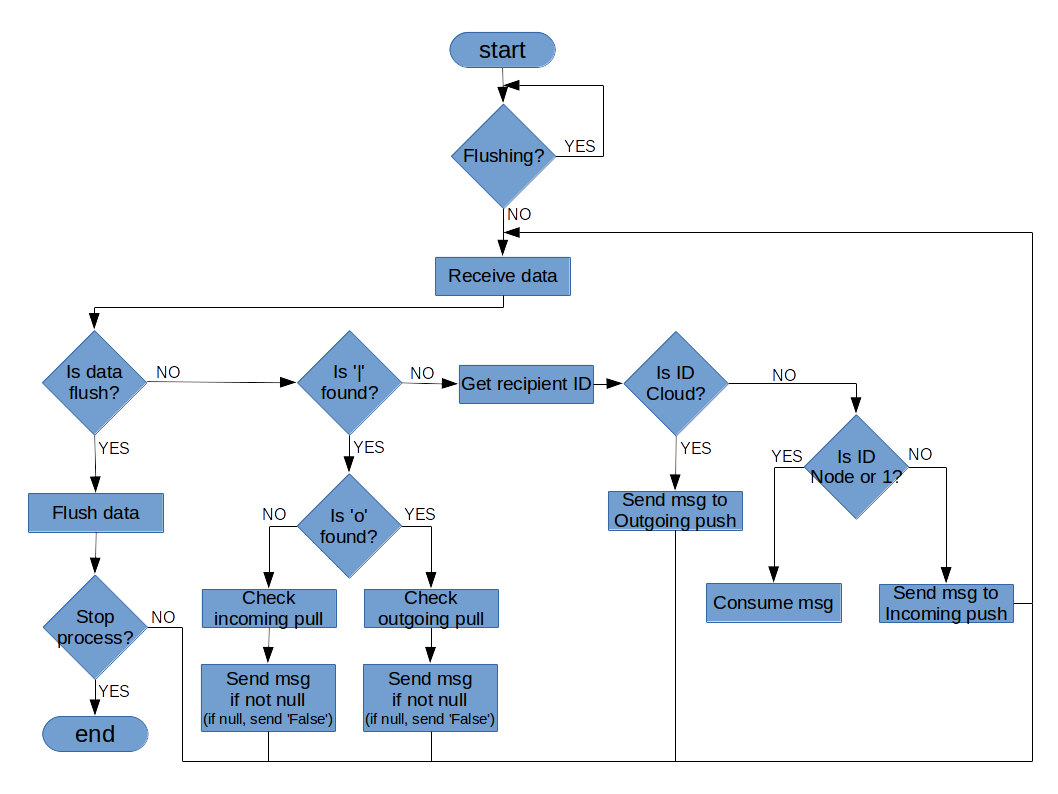
\includegraphics[width=\textwidth]{datacache_flowchart.png}

\textbf{TODO: data cache is consuming Waggle messages sent to the nodecontroller. We need to take the consumption part out from the data cache and put the part 
somewhere in internal communication.}

\subsection{Routing}
\label{routing}

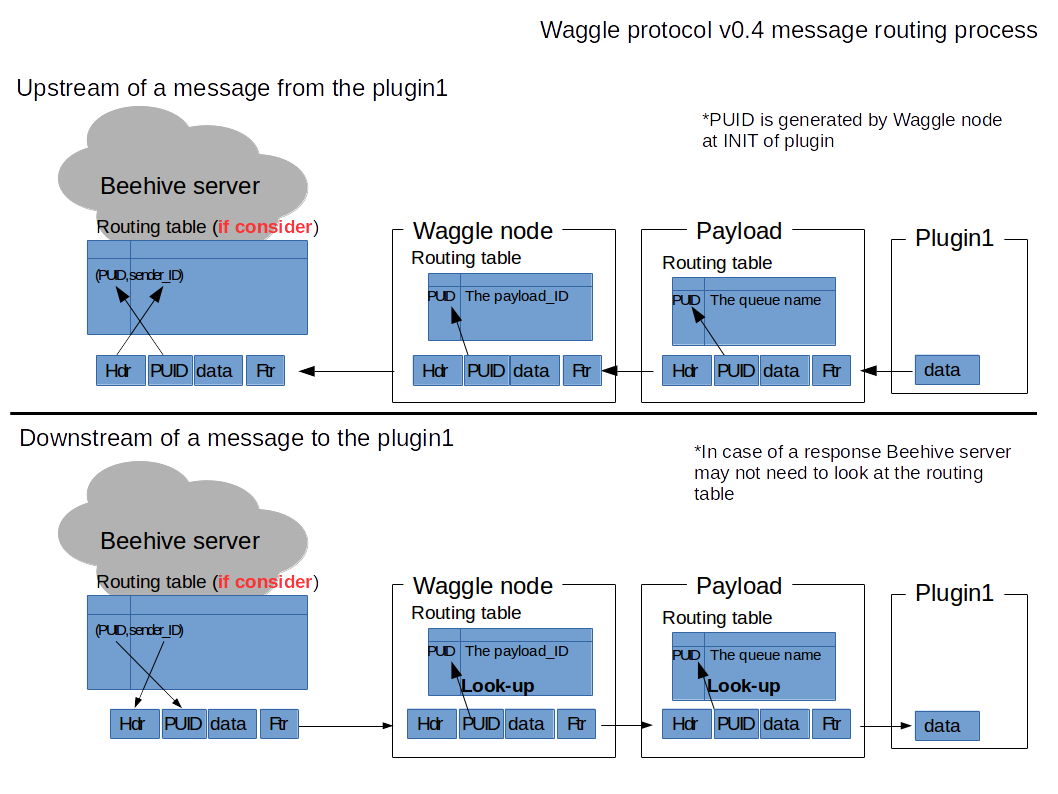
\includegraphics[width=\textwidth]{routing_process.png}

\noindent
Routing table is used to distribute Waggle messages to all connected components (i.e., payloads, plugins). All incoming Waggle messages 
that have $PUID$ in $Ext\_header$ set are consiered to be routed (Waggle messages that do not set $PUID$ are excluded for this route and will be 
consumed by the node). In the table, primary key is a unique number generated by nodecontroller and is mapped with routing information. An example of the 
routing table would look like,

\begin{center}
    \rowcolors{1}{rahmen!8}{white}
    \begin{tabular}{ | p{2cm} | p{3cm} | p{8cm} |}
    \hline
    \hline
    \textbf{ID} & \textbf{ROUTING} & \textbf{Meta} \\ \hline \hline
    0 & NODE\_ID & ``\{`name':`example\_plugin', `ver':`0.3', ... \}'' \\  \hline
    1 & PAYLOAD1\_ID & ``\{`name':`airsensor', `ver':`0.4', ... \}'' \\  \hline
    2 & PAYLOAD2\_ID & ``\{`name':`example\_plugin', `ver':`0.3', ... \}'' \\  \hline
    \end{tabular}
\end{center}

In this example ID 0 seems that it is a plugin attached to the nodecontroller. When a Waggle message with the ID 0 comes to the nodecontroller it will go to 
the `system\_receive' plugin running on the same node. ID 1 is also a plugin attached to the payload1 so the nodecontroller needs to send the message to the 
payload1 first and the message will be routed again in the payload1.

\subsubsection{Registration for routing}

The registration request ($Msg\_Mj\_Type$ `r' and $Msg\_Mj\_Type$ `r') will be sent to the parent node and will also be consumed at the node that has routing 
table. If the requestor is already in the routing table, a response message with the corresponding ID will be sent. When a registered plugin lost its 
ID or rebooted with a different instance a new ID will be assigned to the plugin. \textbf{TODO: we will need to clean up the routing table for some IDs that 
seem never used}

\subsubsection{Flushing the routing table to the server}

When the nodecontroller boots up it may wait until it gets a number of registration requests from attached plugins or payload nodes along with their meta data 
(e.g., name, version, instance, etc.). At a certain point of time, the nodecontroller needs to flush the routing table with all the meta data to the Beehive 
server so that the server could respond requests and sometimes send a message to the plugin registered in the routing table.

\subsubsection{Communication with Beehive server}

When connection is available to the server, nodecontroller pushes Waggle messages piled in the Data\_cache. All the outgoing Waggle messages will get the same
$S\_Uniq\_ID$ set by the ID of the nodecontroller so that the server only takes care of nodes, not plugins nor payloads.


\section{Payload}

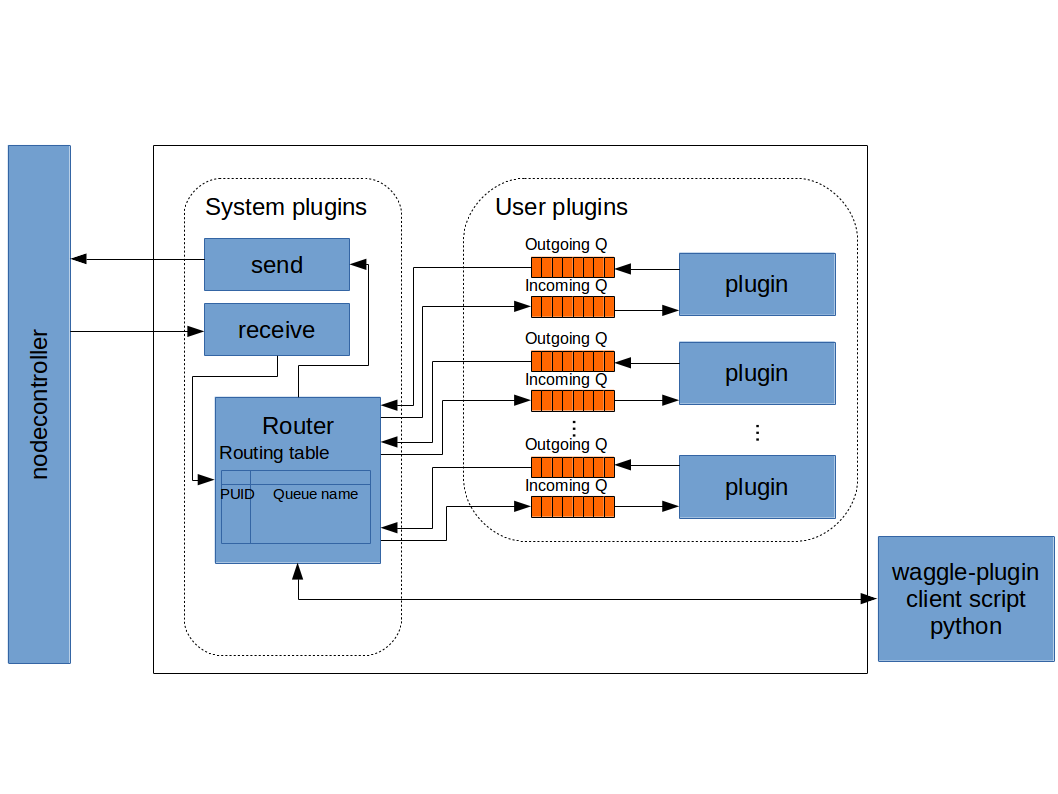
\includegraphics[width=\textwidth]{payload_diagram.png}




\subsection{Plugins}

\subsubsection{System plugins}

\begin{itemize}
\item {System\_send: } packetizes JSON data into Waggle message. Waggle messages are sent to attached parent node via TCP/IP.
\item {System\_receive: } receives Waggle messages, check CRC, de-serialize the message using JSON, and send it to system\_router plugin. 
\item {System\_router: } routes JSON data. This plugin holds routing table to distribute messages properly. For the details of the routing table, refer to 
\ref{routing}.
\end{itemize}

\subsubsection{User plugins}



The data types used in JSON are listed below.
\label{json_keywords}
\begin{center}
    \rowcolors{1}{rahmen!8}{white}
    \begin{tabular}{ | p{3cm} | p{3cm} | p{8cm} |}
    \hline
    \hline
    \textbf{KEYWORD} & \textbf{MEANING} & \textbf{NOTE} \\ \hline \hline
    msg\_mj\_type & Major operation & One char \\  \hline
    msg\_mi\_type & Minor operation & One char \\  \hline
    s\_puid & Plugin/Payload unique identifier & Sender's PUID  \\  \hline
    p\_puid & Plugin/Payload unique identifier & Recipient's PUID  \\  \hline
    meta & Meta data & Dictionary-type information (plugin name, version, instance, etc.)  \\  \hline
    data & Data & Dictionary-type data  \\  \hline
    rec & Recipient & Specify recipient (Default is Beehive) \\ \hline
    snd\_s & Sender's sequence number & Sequence number of the sender (optional) \\ \hline
    resp\_s & Responder's sequence number & Sequence number of the responder (optional) \\ \hline
    snd\_ss & Sender's session number & Session number of the sender (optional) \\ \hline
    resp\_ss & Responder's session number & Session number of the responder (optional) \\ \hline
    error & Error message & Error message when occur (optional) \\ \hline
    \end{tabular}
\end{center}

When JSON contains `error' plugins need to react to it appropriately.

\subsubsection{Communication}

All communications between system\_router and plugins are through JavaScript Object Notation (JSON).

\subsubsection{Registration}

A plugin should maintain a plugin unique identifier (PUID) generated by the nodecontroller the plugin attached to. If the plugin cannot find the PUID (either 
the first time or missing), the plugin can request a PUID by sending a registration request to the nodecontroller. As an example would be,

\begin{framed}
\noindent
\{``mj\_op'':``r'', ``mi\_op'':``r'', ``puid'':uuid.uuid4(), ``meta'':``... plugin name, version, instance...''\}
\end{framed}

For ``tmpID'' use randomly generated ID using uuid package in Python. This ``tmpID'' will only be used until the plugin gets PUID from the nodecontroller. The 
PUID should be properly maintained by the plugin (e.g., in a file) and should not be altered.

\subsubsection{Listener}

If a plugin needs to get data from outside (e.g., the Beehive server or nodes), the plugin should assign an asynchronous listener and make the listener 
attached to the incoming queue. For the format of incoming message, refer to \ref{json_keywords}.
\section{Beehive server}

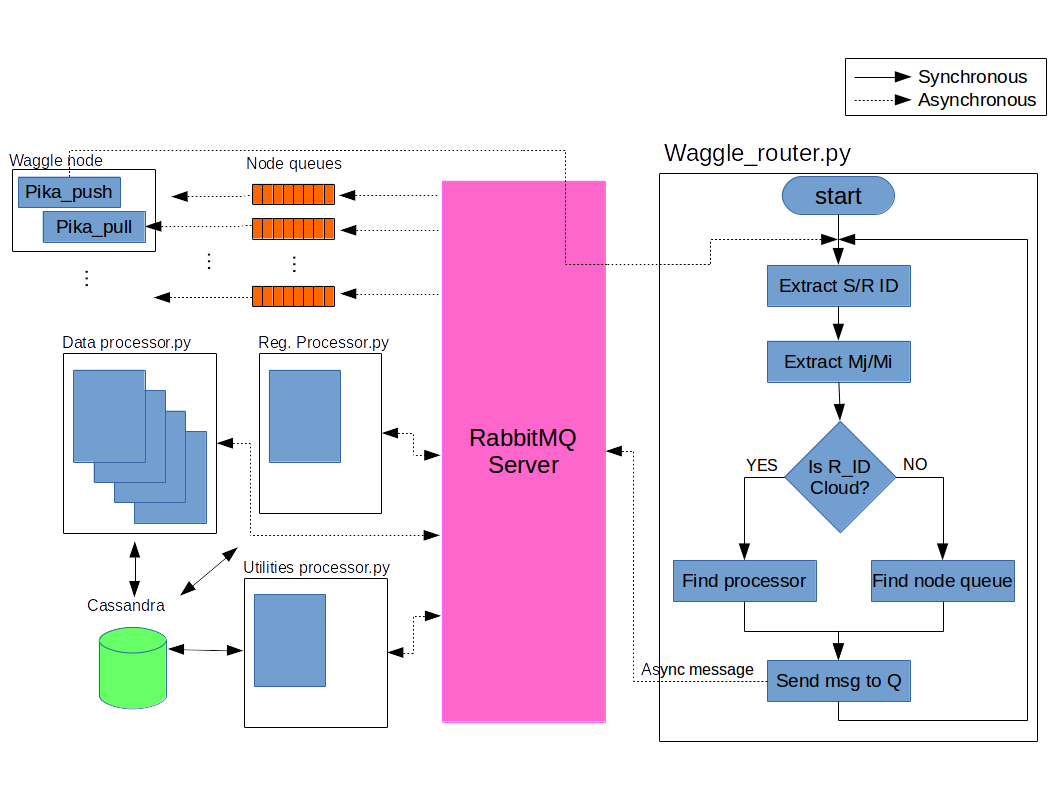
\includegraphics[width=\textwidth]{beehive_diagram.png}

\subsection{Store data}

After unpacking Waggle message, the actual payload message is JSON type. Server process should handle JSON data to pull values and store them in the database. 
JSON data consist of the following format. for now the format is based on `sensor\_table' scheme.

\begin{framed}
\noindent
node\_id, date, plugin\_id, plugin\_version, plugin\_instance, timestamp, sensor, sensor\_meta, data
\end{framed}

\textbf{TODO: Do we need to look up the routing table in the server everytime when a Waggle message comes to the 
server?}



\end{document}
